\subsection{Completed reduced extension and the multiconfigurational limitation}
\begin{table}[!htbp]
\centering\small
\caption{Completed reduced extension: MAE (eV) on the same geometries and assigned states. F and Q denote the two corrected GFN2 parents; TDA mean is their arithmetic spectral average. This adapted set is separate from the original 19-state cohort.}\label{tab:extension}
\begin{tabular}{lrrrrr}
\toprule
Family & $N$ & OO 50/50 & TDA-F & TDA-Q & TDA mean \\
\midrule
All & 14 & 0.492 & 1.013 & 0.261 & 0.611 \\
$n\pi^*$ & 5 & 0.193 & 0.592 & 0.142 & 0.311 \\
$\pi\pi^*$ & 5 & 0.954 & 1.409 & 0.417 & 0.913 \\
CT & 3 & 0.187 & 0.890 & 0.244 & 0.539 \\
Rydberg & 1 & 0.598 & 1.499 & 0.129 & 0.814 \\
\bottomrule
\end{tabular}
\end{table}

The completed 14-state extension gives an MAE of 0.492~eV for the original single-CSF 50/50 model, compared with 0.261~eV for TDA-Q, 1.013~eV for TDA-F, and 0.611~eV for their arithmetic mean. The five $\pi\pi^*$ states account for an OO MAE of 0.954~eV; cyclopentadiene, furan, and phthalimide are overestimated by 1.746, 1.444, and 1.269~eV, respectively. These results do not support a general accuracy advantage over TDA. Assignment success and predictive accuracy must be assessed separately.

The leading squared NTO singular values of these three fixed projected transitions are 0.544, 0.533, and 0.754. A single excited singlet CSF cannot represent the orthogonal transition pairs carrying the remaining weight. As a development test, an orthonormal set of singlet excitation CSFs is combined by diagonalizing a small state-interaction matrix with unchanged ROKS diagonal energies and bare Slater--Condon off-diagonal couplings,
\begin{equation}
 H_{ii}=2E_{M_i}-E_{T_i},\qquad
 H_{ij}=2(h_ip_i|h_jp_j)-(h_ih_j|p_ip_j),\quad i\ne j.
\end{equation}
The use of a small configuration space with DFT-informed diagonal energies is motivated by minimal-active-space multistate DFT.\cite{masmsdft2021} That approach optimizes determinant orbitals separately and uses nonorthogonal state interaction; the present common-orbital, orthonormal-CSF construction is a different approximation. This defines a new approximate multistate energy, with a spin-pure wavefunction and analytic CI-eigenvector response. The off-diagonal operator is unscaled bare exchange/Coulomb, whereas the diagonal response retains $\lambda=0.9$; it differs from the TDA kernel. No energy offset or fitted interaction multiplier is introduced. The two parents retain equal weights. The present test chooses the smallest NTO rank containing 95\% of the fixed transition norm, capped at four. All labels are already exposed at this development stage.

\begin{table}[!htbp]
\centering\small
\caption{Exposed-label minimal-CSF development trial. Off-diagonal bare Slater--Condon couplings and a 95\% NTO-norm rank rule define a new approximate functional. The $n\pi^*$ control invalidates a universal repair claim.}\label{tab:multicsfdev}
\begin{tabular}{llrrrr}
\toprule
Molecule & Family & Rank & TBE & Original OO & Trial OO \\
\midrule
Adenine & $\pi\pi^*$ & 2 & 5.191 & 5.449 & 5.191 \\
Cyclopentadiene & $\pi\pi^*$ & 2 & 6.451 & 8.197 & 6.720 \\
Furan & $\pi\pi^*$ & 2 & 6.530 & 7.974 & 6.674 \\
Phthalimide & $\pi\pi^*$ & 2 & 4.600 & 5.869 & 4.946 \\
Aza-naphthalene & $n\pi^*$ & 3 & 5.346 & 5.279 & 2.839 \\
Bimane\_Syn & $\pi\pi^*$ & 1 & 3.964 & 3.911 & 3.911 \\
\bottomrule
\end{tabular}
\end{table}

On the five $\pi\pi^*$ examples this trial reduces the MAE from 0.954 to 0.162~eV, and all eight newly optimized multi-CSF parent points pass the available-root identity audit. However, the same rank rule introduces three CSFs for the aza-naphthalene $n\pi^*$ state and lowers its prediction from 5.279 to 2.839~eV against 5.346~eV. The 95\% prescription therefore cannot be promoted as a transferable correction; possible correlation double counting and the treatment of weak configurations remain unresolved. The Rydberg-control attempts and blocked optimization paths are retained in the development archive. Replacing the interaction with the native GFN2 screened charge kernel has so far only been examined at fixed orbitals and does not constitute a validated alternative.

An independent HF-limit check contracts the same CSFs with a fermionic Hamiltonian and verifies $S^2=0$. Finite rotations test the complete analytic orbital Hessian, including CI response. A frozen co-rotating orthonormal-AO transport defines the experimental nuclear surface explicitly. For the furan F parent, two reoptimized finite-difference columns agree with its analytic nuclear Hessian within $2.2\times10^{-8}$~\Eh/bohr$^2$. For the two-parent candidate, the individual-cosine constraint Jacobian is singular at the furan anchor; its second-order information cannot be discarded. A different, regular manifold preserves the full active cross-overlap matrix exactly through common metric-orthogonal rotations and independent spectator rotations. At independently stationary anchors its analytic response is a projected coupled Hessian with complete CI and orbital response. Two finite-difference columns of the furan total excited energy, including native-ground restoration and subtraction of both corrected ground references, agree within $2.3\times10^{-8}$~\Eh/bohr$^2$. These calculations reuse all completed ground checkpoints. The full-frame constraint defines a stricter experimental PES than the original individual-cosine model. Off anchor, the implementation includes common/private product-chart terms and mixed spectator-gauge curvature. Two columns of the constrained parent-mean Hessian at a displaced furan geometry also agree within $2.3\times10^{-8}$~\Eh/bohr$^2$, despite individual parent orbital residuals around $2.3\times10^{-4}$~\Eh. Complete molecular Hessian-column checks, broader off-anchor qualification, frequency accuracy and automatic LINK/APOC integration of this new functional remain open.

A second development proposal defines the active rank by the effective number of transition pairs rather than a cumulative norm cutoff. With normalized NTO weights $w_i=\sigma_i^2/\sum_j\sigma_j^2$, let
\begin{equation}
 N_{\mathrm{pair}}=\frac{1}{\sum_i w_i^2},\qquad
 r=\left\lfloor N_{\mathrm{pair}}+\tfrac12\right\rfloor.
\end{equation}
No excitation energy or state-family label enters this rule. It selects rank two only for cyclopentadiene ($N_{\mathrm{pair}}=1.988$), furan (2.011), and phthalimide (1.595); the other 11 states have rank one and reuse the identical original single-CSF functional. Existing stationary parents suffice, with no new energy correction or interaction parameter. The resulting vertical development MAE is 0.228~eV over all 14 states and 0.214~eV over the five $\pi\pi^*$ states. All $n\pi^*$, CT, and Rydberg values remain unchanged. This is a proposed solution to weak-pair overcorrelation in the cumulative-cutoff trial, not an independently validated universal prescription: the choice was motivated after seeing that trial. Phthalimide lies only 0.095 above the nearest half-integer rank boundary, making anchor and rank sensitivity a required further test. Rydberg accuracy remains limited.

\begin{figure}[!htbp]
\centering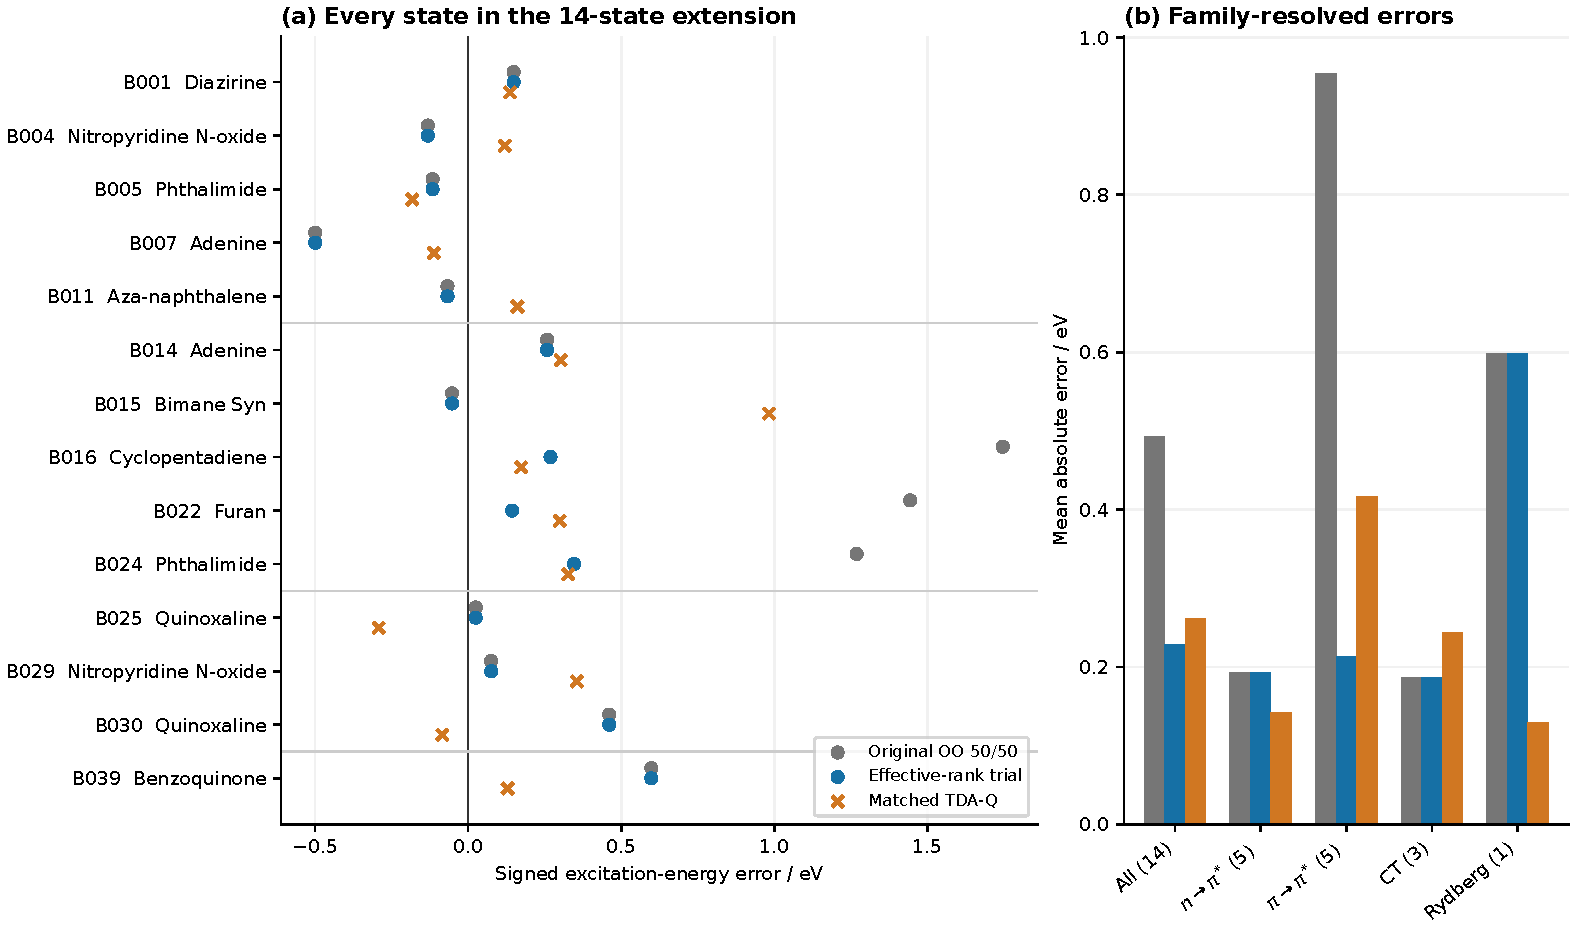
\includegraphics[width=\linewidth]{figures/multicsf_development.pdf}
\caption{Effective-rank multi-CSF development candidate on the completed extension. (a) Every state error; (b) family MAEs. The rank criterion changes only three $\pi\pi^*$ predictions and leaves the other 11 values unchanged. Labels were already exposed, and this is not an independent validation. The adverse aza-naphthalene result of the separate 95\% rule is retained in Table~\ref{tab:multicsfdev}. TDA-Q is computed on the corrected GFN2 ground orbitals.}\label{fig:multicsfdev}
\end{figure}

The present rank-selection protocol uses the archived DFT reference transition amplitudes. These are reused during the semiempirical surface calculation, but are part of its reference preparation cost. A stand-alone selection using ground-state information alone has not been demonstrated for this candidate.
